\chapter{Problem analysis and requirements}
\label{ch:problem-analysis}

This chapter investigates the different use cases associated with cinema management and discusses potential pitfalls in the design of a generic solution. To gain a comprehensive understanding of the problem space, detailed use cases are analyzed and requirements are derived therefrom. A list of requirements is presented, which will serve as a basis for the conceptual design in the following chapter.

\section{Use-cases}\label{sec:use-cases}

To further comprehend the necessary functionality for \gls{g:cms}, a use case diagram was developed based on the client's specifications \cite[1--2]{IIS2-ass}. This diagram visually depicts the critical interaction points between users and \gls{g:cms}, as well as the provided configuration interface for the cinema owner. By providing a visual representation, the diagram facilitates seamless communication among all parties involved and aids in deriving requirements.

\begin{figure}[H]
    \centering
    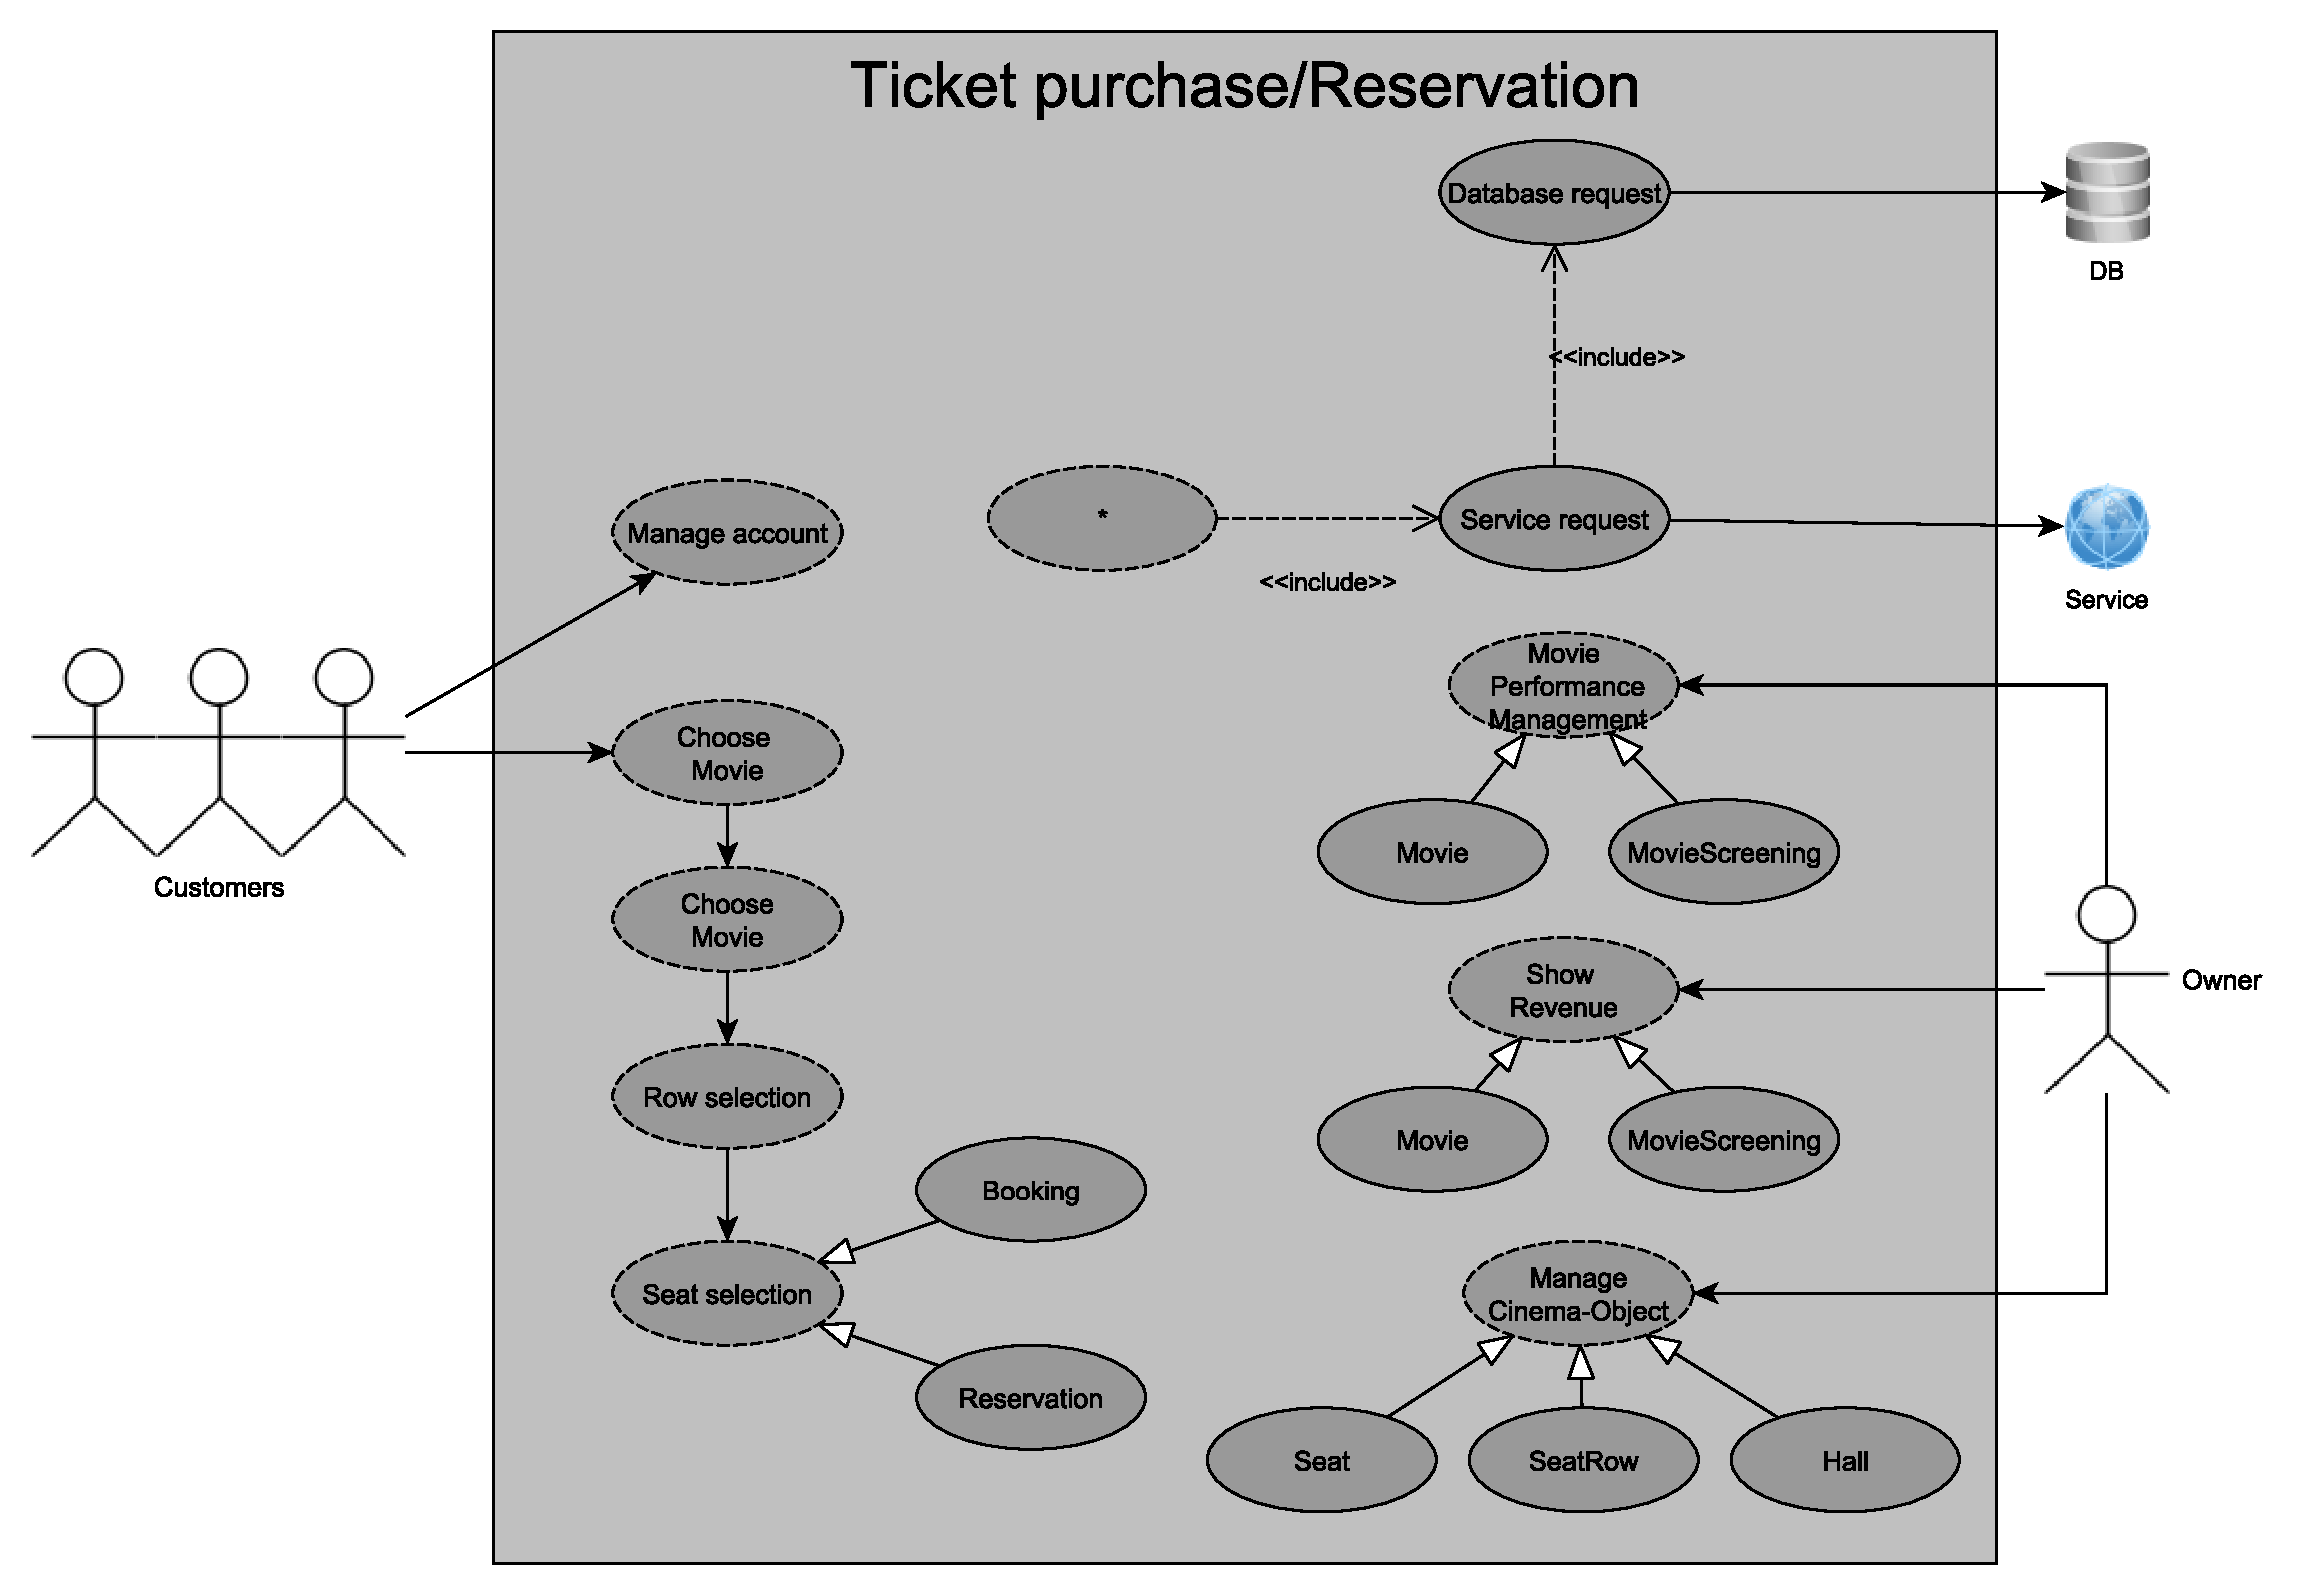
\includegraphics[width=\textwidth]{images/iis-use.case-new}
    \caption{Simplified use-case diagram of actor interaction with \gls{g:cms}.}
    \label{fig:use-cases}
\end{figure}

The simplified\footnote{To maintain brevity and clarity, activities involving \gls{a:api} requests have been indicated with dashed borders, rather than explicitly modeling \inlinecode{<<include>>} relationships. Nonetheless, the underlying semantics remain unchanged.} use-case diagram in Figure \ref{fig:use-cases} illustrates two primary interactions: one between the cinema owner and the proposed \gls{g:cms} solution, and the other between customers and the system.

The cinema owner can manage various aspects of the cinema through the \gls{g:cms}, including cinema halls, seats, seat rows, movies, and movie screenings. In this context, \enquote{manage} refers to the \gls{a:crud} operations. These cinema-infrastructure-related tasks are commonly denoted as \inlinecode{management} activities throughout this document. Additionally, the owner can view revenue generated from movies and individual screenings. These operations are categorized as administrative or \inlinecode{admin} use-cases.

Conversely, customers can create and manage accounts, reserve or book seats for movies, and view or cancel their reservations. They can select a movie, choose a specific screening, and pick their desired row and seat. Afterward, customers can either book the seat immediately or reserve it for booking later. The group of use-cases related to customer interactions is referred to as \inlinecode{user} use-cases.

While the diagram offers a fundamental overview of the \gls{g:cms} solution's desired functionality, it does not provide specific details. Consequently, the following section delves deeper into the technical implications of the various use-cases, deriving requirements accordingly.

A more detailed description of different scenarios and use-cases written in natural language is presented in \cref{apx:sec:use-cases}.

\section{Requirements}
\label{sec:requirements}

This section delves into the use-cases outlined in \cref{sec:use-cases}, with the aim of extracting requirements for a \gls{g:cms} prototype. To achieve this, the subsequent subsections examine the challenges and constraints associated with the various use-cases, along with their corresponding requirements.

\subsection{Interaction with \glsentrytext{g:cms}}\label{sec:req-interaction}
A fundamental question arising from the use-cases outlined in \cref{sec:use-cases} concerns the method of how an actor interacts with the proposed \gls{g:cms} solution. Specifically, whether a \gls{a:gui} or a \glsfull{a:cli} should be employed for system interaction. The primary distinction between these two approaches lies in \glspl{a:gui} utilizing visual cues to convey information to users, whereas \glspl{a:cli} rely on text-based commands for input and output of information.

The client has indicated that a full \gls{a:gui} is not required for the \gls{g:cms} prototype, suggesting that a \gls{a:cli} would suffice \cite[2]{IIS2-ass}. Nevertheless, considering that software solutions are often evaluated based on the user experience they offer, the development team has opted to prioritize delivering a user-friendly interface. This requirement entails that the \gls{g:cms} client application should be as accessible as a \gls{a:gui}, which can be accomplished by providing a \gls{a:cli} with a comprehensive feature set.

\subsection{Communication Between Actors and \glsentrytext{g:cms}}\label{sec:req-protocol}

Furthermore, the client specified that the \gls{g:cms} should be accessible to both the owner and customers through a client-server architecture \cite{IIS2-ass}. As a result, it is essential to define the communication protocol to be employed by the \gls{g:cms} \gls{a:api}.

Apart from specifying network-based communication, no additional constraints have been imposed on the selection of the communication protocol. Consequently, the development team has opted to use the \gls{a:http} 1.1 specification, implementing a \inlinecode{REST}ful \gls{a:api} that employs \gls{a:json} for data serialization. This choice is grounded in the widespread use of the \inlinecode{REST} architecture for \glspl{a:api}, ensuring seamless interoperability with other software components that may extend the \gls{g:cms} solution in future development efforts. The decision for \gls{a:json} for data serialization is based on its status as a commonly used, standardized data-exchange format for \glspl{a:api}, increasing the likelihood of the client's familiarity with it. Additionally, its human-readable nature proves particularly valuable during development, facilitating easy debugging of the \gls{a:api}. Finally, as the \gls{a:json} format is a subset of the JavaScript language, which most web browsers natively support, it offers the potential for future development of a web-based user interface without necessitating extra dependencies.

\subsection{Client Portability}\label{sec:req-client-portability}

To guarantee a seamless user experience, the \gls{g:cms} client application must be accessible across various platforms, ensuring portability across operating systems and architectures. Ideally, it should be a standalone executable file without any additional dependencies.

Considering these requirements, the development team chose C\#/.NET as the programming language for the \gls{g:cms} client application. This decision was based on C\#/.NET's ability to be packaged as a self-contained executable file, enabling native compilation into architecture-specific binaries. Consequently, the client application can run on compatible systems without additional runtime or framework dependencies. The C\#/.NET ecosystem also offers a diverse set of libraries for \gls{a:cli}-development, such as \inlinecode{System.Commandline}, allowing for shorter development times and less boilerplate for command parsing.

\pagebreak

\subsection{Summary of Requirements}
\label{sec:requirements-summary}

The investigation of the challenges elucidated in the use cases and the constraints associated therewith have led to the establishment of the following prerequisites for the proposed \gls{g:cms} solution. These requirements will serve as a basis for the conceptual design in the following chapter.

\renewcommand{\arraystretch}{1.25}
\begin{table}[H]
    \centering
    \caption{Summary of requirements for \gls{g:cms}.}
    \label{tab:requirements}
    \begin{tabular}{l|p{0.75\textwidth}}
        \toprule
        Requirement & Description \\ \midrule
        \requirementdefshort\label{req:use-cases}  & \gls{g:cms} must cover the use-cases discussed in \cref{sec:use-cases} and \cref{apx:sec:use-cases}. \\ \hline
        \requirementdefshort\label{req:model-requirements}  & \gls{g:cms} must comply with all model-specific requirements specified in \cref{apx:ch:extended-analysis}. \\ \hline
        \requirementdefshort\label{req:client-server} & \gls{g:cms} must utilize the client-server architecture, allowing multiple concurrent clients to access its services \cite[2]{IIS2-ass}. \\ \hline
        \requirementdefshort\label{req:database} & A database engine must be used to persist cinema data. \\ \hline
        \requirementdefshort\label{req:server} & The \gls{g:cms} server must be written in as a Java application complying with the principles of model driven development \cite[1]{IIS2-ass}. \\ \hline
        \requirementdefshort\label{req:mps} & \gls{a:mps} by JetBrains must be used to generate the Java source code for data access layer and the \gls{a:sql} \gls{a:ddl} statements required for the database schema \cite[1]{IIS2-ass}. \\ \hline
        \requirementdefshort\label{req:mysql} & \gls{g:cms} data must be persisted in a MySQL database \cite[4]{IIS2-ass}. \\ \hline
        \requirementdefshort\label{req:isolation} & Database access must be performed in a thread-safe and isolated manner \cite[2]{IIS2-ass}. \\ \hline
        \requirementdefshort\label{req:api} & The server must provide a \gls{a:rest}ful \gls{a:json} \gls{a:api} for the client application to communicate with, as established in \cref{sec:req-protocol}. \\ \hline
        \requirementdefshort\label{req:client-access} & The client application must be able to connect to the server via a \gls{a:rest}ful \gls{a:json} \gls{a:api} using \gls{a:http} 1.1 as the underlying protocol (see \cref{sec:req-protocol}). \\ \hline
        \requirementdefshort\label{req:client-cli} & A \gls{a:cli} must be provided for user interaction within the client application, as established by \cref{sec:req-interaction}. \\ \hline
        \requirementdefshort\label{req:client-firendly-cli} & Although a \gls{a:cli} is sufficient for the prototype, usability and user experience should be a priority for the development, as established by \cref{sec:req-interaction}. \\ \hline
        \requirementdefshort\label{req:client-portability} & The client application must be capable of being published as a self-contained executable, guaranteeing portability without reliance on any additional runtime environment for installation. This requirement was established in \cref{sec:req-client-portability} \\ 
        \bottomrule
    \end{tabular}
\end{table}
\renewcommand{\arraystretch}{1}